\section{Прочие тестовые статистики}

Перестановочные тесты точны при применении любой тестовой статистики $\hat{\theta}$. Верхняя правая часть рисунка 15.1 отображает разницу 15\% средних
\begin{equation}
	\hat{\theta} = \bar{z}_{0.15} - \bar{y}_{0.15}.
\end{equation}

\noindent
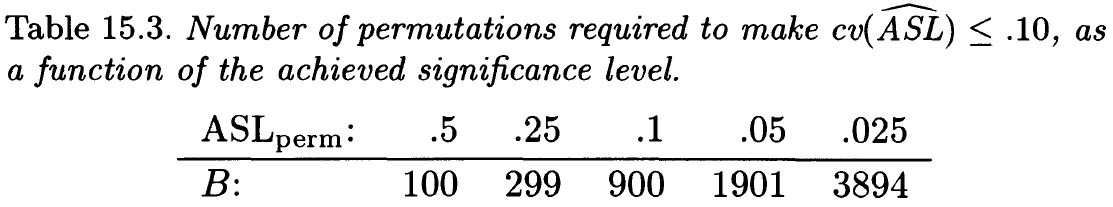
\includegraphics[width=\textwidth]{15/t15.3}
\newline

\noindent Нижняя левая часть рисунка отобрадает разницу 25\% средних значений, а нижняя правая часть --- разницу медиан. Одинаковое число $B = 1000$ перестановочных векторов $\bf{g}^*$ используется во всех четырех частях рисунка, изменяется только статистика $\hat{\theta}^* = S(\bf{g}^*, \bf{v})$. Все четыре значения $\widehat{\text{ASL}}_{\text{perm}}$, 0.132, 0.138, 0.152 и 0.172 согласуются с принятием нулевой гипотезы $F = G$.

Тот факт, что каждое $\hat{\theta}$ приводит к точному $\text{ASL}_{\text{perm}}$, не означает, что все $\hat{\theta}$ являются одинаково хорошей тестовой статистикой. «Точность» означает, что эти $\text{ASL}_\text{perm}$ не будут иметь тенденцию быть обманчиво маленькими, когда $H_0$ истинно, как указано в (15.22). Однако, если $H_0$ ложно, если экспериментальная группа дает действительно лучшие результаты, чем контрольная, тогда мы хотим, чтобы $\text{ASL}_\text{perm}$ был маленьким. Это свойство статистического теста называется мощностью. Наказанием за выбор плохой тестовой статистики $\hat{\theta}$ является малая мощность --- мы не получаем большой вероятности отклонить $H_0$, когда оно ложно. Мы скажем немного больше о выборе $\hat{\theta}$ в обсуждении бутстрепа, который завершает эту главу.

Глядя на Таблицу 2.1, эти две группы, кажется, различаются больше по дисперсии, чем по средним. Отношение оценочных дисперсий составляет около 2.5
\begin{equation}
	\hat{\sigma}^2_z / \hat{\sigma}^2_y = 2.48.
\end{equation}
Является ли эта разница значимой или это просто артефакт небольшого размера выборки?

Мы можем ответить на этот вопрос с помощью перестановочного теста. На рисунке 15.2 показано 1000 перестановочных репликаций
\begin{equation}
	\hat{\theta} = \log (\hat{\sigma}^2_z/\hat{\sigma}^2_y).
\end{equation}
(Логарифм не влияет на перестановочные результаты). 152 из 1000 значений $\hat{\theta}^*$ превышают $\hat{\theta} = \log(2.48) = 0.907$, что дает $\widehat{\text{ASL}}_{\text{perm}} = 0.152$. И снова нет оснований отвергать нулевую гипотезу $F = G$. Обратите внимание, что мы \textit{могли} отклонить $H_0$ с помощью этой $\hat{\theta}$, даже если мы не отклонили ее с помощью $\hat{\theta} = \bar{z} - \bar{y}$. Этот $\hat{\theta}$ измеряет отклонения от $H_0$ другим способом, нежели $\hat{\theta}$ на рисунке 15.1.

Статистика $\log (\hat{\sigma}^2_z/\hat{\sigma}^2_y)$ существенно отличается от $\bar{z} - \bar{y}$. Лечение было разработано для увеличения времени выживания, поэтому мы ожидаем, что $\bar{z} - \bar{y}$ будет больше нуля, если лечение работает, то есть если $H_0$ ложно. С другой стороны, у нас нет априорных оснований полагать, что $\hat{\theta} = \log (\hat{\sigma}^2_z/\hat{\sigma}^2_y)$ будет больше нуля, а не меньше нуля, если $H_0$ ложно. Другими словами, нас бы так же интересовал результат $\hat{\theta} = -\log(2.48)$, как и результат $\hat{\theta} = \log(2.48)$.

\noindent
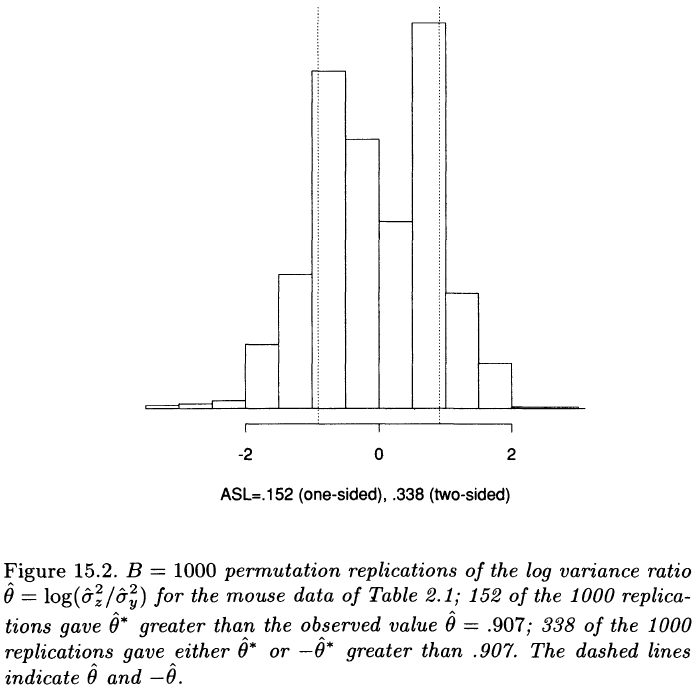
\includegraphics[width=\linewidth]{15/f15.2}
\newline

В этой ситуации обычно вычисляется \textit{двусторонний} ASL, а не \textit{односторонний} ASL (15.4). Это делается путем сравнения абсолютного значения $\hat{\theta}^*$ с абсолютным значением $\hat{\theta}$
\begin{equation}
	\widehat{\text{ASL}}_{\text{perm}}(\text{двусторонний}) = \# \{ |\hat{\theta}^*(b)| > |\hat{\theta}| \}/B.
\end{equation}
Точно так же мы подсчитываем случаи, когда либо $\hat{\theta}^*$, либо $-\hat{\theta}^*$ превосходят $|\hat{\theta}|$. Двусторонний ASL всегда больше одностороннего ASL, что дает меньше оснований для отклонения $H_0$. Двусторонний тест по своей сути более консервативен. Для данных о мышах, статистика (15.25) дала двусторонний ASL в размере 0.338.

Идея теста значимости может быть сформулирована следующим образом: мы ранжируем все возможные наборы данных $\bf{x}$ в соответствии с тем, насколько сильно они противоречат нулевой гипотезе $H_0$; тогда мы отклоняем $H_0$, если $\bf{x}$ входит в 5\% (или 10\%, или 1\% и т.д., как в (15.5)) набора данных, которые наиболее сильно противоречат $H_0$. Определение ASL в (15.4) сводится к измерению противоречия в соответствии с размером $\hat{\theta}(\bf{x})$, большие значения $\hat{\theta}$ подразумевают большие доказательства против $H_0$. Иногда, однако, мы считаем, что большие отрицательные значения $\hat{\theta}$ так же хороши, как большие положительные значения для дискредитации $H_0$. Так было в (15.25). Если так, нам необходимо принять это во внимание при определении 5\% набора данных, которые наиболее сильно противоречат $H_0$. Это точка в определении (15.26) двустороннего ASL.

Есть много других ситуаций, в которых нам нужно быть осторожными при ранжировании свидетельств против $H_0$. Предположим, например, что мы запускаем четыре перестановочных теста, показанных на рисунке 15.1, и решаем выбрать тот, у которого наименьшее значение ASL, в данном случае $\widehat{\text{ASL}} = 0.132$. Тогда мы действительно ранжируем доказательства по $\bf{x}$ против $H_0$ согласно статистике
\begin{equation}
	\hat{\varphi}(\textbf{x}) = \min_k \{ \widehat{\text{ASL}}_k \},
\end{equation}
где $\widehat{\text{ASL}}_k$ --- перестановочный ASL для $k$-й статистики $\hat{\theta}$ для $k = 1, 2, 3, 4$. Малые значения $\hat{\varphi}$ сильнее противоречат $H_0$. \textit{Неверно}, что, наблюдая $\hat{\theta} = 0.132$, перестановочный ASL основанный на $\hat{\varphi}$ равняется 0.132. Более 13,2\% перестановок будут иметь $\hat{\varphi}^* < 0.132$ из-за минимизации в определении (15.27).

Вот как вычислить правильный перестановочный ASL для $\hat{\varphi}$, используя все 4000 перестановочных репликаций $\hat{\theta}^*_k (b)$ на рисунке 15.1, $k = 1, 2, 3, 4, b = 1, 2, \ldots, 1000$. Для каждого значения $k$ и $b$ определяют
\begin{equation}
	A^*_k(b) = \dfrac{1}{1000} \sum\limits_{i=1}^{B} I_{\{\theta^*_k(i) \geq \hat{\theta}^*_k(b)\}},
\end{equation}
где $I_{\{ \cdot \}}$ --- индикаторная функция. Итак, $A^*_k(b)$ --- это доля значений $\hat{\theta}^*$, превышающих $\hat{\theta}^*_k(b)$. Тогда пусть
\begin{equation}
	\hat{\varphi}^*(b) = \min_k \{ A^*_k (b) \}.
\end{equation}
Это не очевидно, но верно, что $\hat{\varphi}^*(b)$ являются подлинными перестановочными репликациями, (15.27), поэтому перестановочные ASL для $\hat{\varphi}$ есть
\begin{equation}
	\widehat{\text{ASL}}_{\text{perm}} = \# \{ \hat{\varphi}^*(b) \leq \hat{\varphi} \} / 1000.
\end{equation}
На рисунке 15.3 показана гистограмма 1000 значений $\hat{\varphi}^*(b)$. 167 из 1000 значений меньше $\hat{\varphi} = 0.132$, что дает перестановочный ASL = 0.167.